\documentclass[assd_tp2_main.tex]{subfiles}

\begin{document}

\section{Síntesis mediante modulación en frecuencia}
\subsection*{Introducción teórica}
La modulación en frecuencia esta dada por:
\begin{eqnarray*}
\textstyle x(t)=A(t)cos(2\pi f_c t+I(t)cos(2\pi f_mt+\phi_m)+\phi_c)
\end{eqnarray*}
Parámetros de la modulación en frecuencia:\\*
\begin{itemize}
\item $f_c$ = frecuencia de la señal portadora\\*
\item $f_m$ = frecuencia de la señal modulante\\*
\item $f_d$ = desviación de la frecuencia (respecto de la portadora)\\*
\item I = $\displaystyle \frac{f_d}{f_m}$ = índice de modulación
\end{itemize}

Por simple inspección se puede ver que si I = 0 la desviación de la frecuencia ($f_d$) debe ser 0 y por ende no hay  modulación en frecuencia. Un caso más interesante es cuando I es mayor que 0, se puede observar que aparecen nuevas componentes espectrales lo que provoca que la energía de la señal sea redistribuida.  
\begin{figure}[H]
\centering
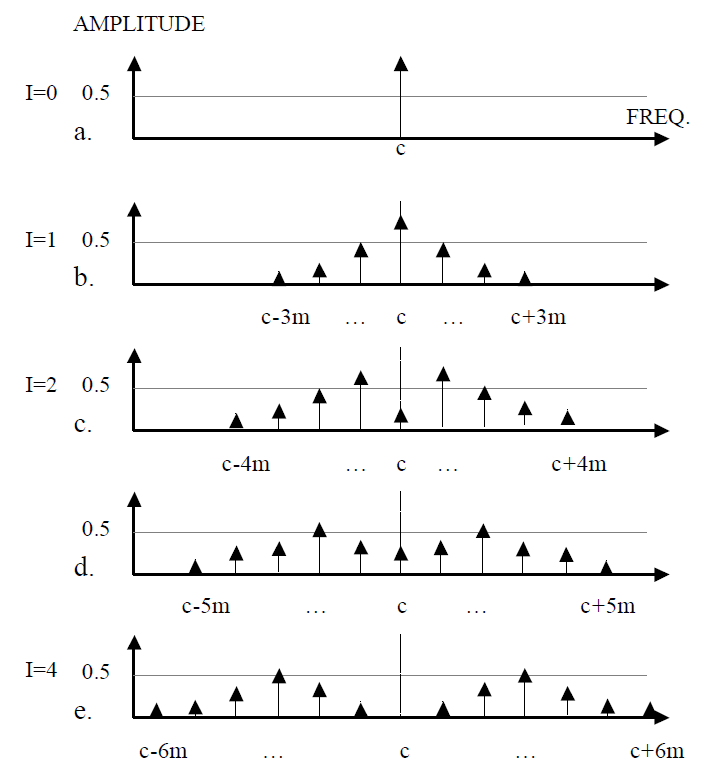
\includegraphics[width=0.4\linewidth]{graficos/EJ4/nuevasfreqs.png}
\caption{Nuevo contenido espectral con I $\neq$ 0}
\label{fig:nuevasfreqs}
\end{figure}
Nota: en el gráfico c = $f_c$ y  m = $f_m$ \\*
Las amplitudes de la portadora y las componentes laterales están dadas por las funciones de Bessel de primera especie y orden n-ésimo,
donde el argumento de la función es el índice de modulacion I ($J_{n}$(I)). \\*
En general, $J_{n}(1)$ representa un coeficiente de escalamiento de amplitud: \\*

$J_{0}(1)\longleftarrow$  para la portadora \\*

$J_{1}(1)\longleftarrow$  para las primeras bandas laterales \\*

$J_{2}(1)\longleftarrow$  para las segundas bandas laterales \\*
\\*
Y así sucesivamente.
Mientras más grande sea el orden de la banda lateral se necesita más índice de modulación para que la misma tenga una amplitud significativa.

\begin{eqnarray*}
\displaystyle BW \approx 2(f_d+f_m)
\end{eqnarray*}

Expresamos a x(t) con funciones de Bessel
\begin{eqnarray*}
\textstyle x(t)=A(t)\cdot \{ \; J_{0}(I)sen(2\pi f_c t) \\*
				+J_1(I)[sen(2\pi(f_c+f_m)t) - sin(2\pi(f_c-f_m)t)] \\*
				+J_2(I)[sen(2\pi(f_c+2f_m)t) + sin(2\pi(f_c-2f_m)t)] \\*
				... \\*
				+J_n(I)[sen(2\pi(f_c+n f_m)t) \pm sin(2\pi(f_c-n f_m)t)] \; \}
\end{eqnarray*}

\begin{figure}[H]
\centering
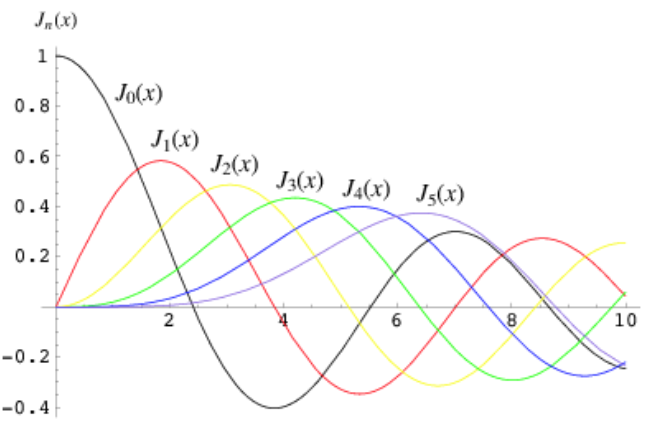
\includegraphics[width=0.4\linewidth]{graficos/EJ4/Bessel.png}
\caption{Funciones de Bessel de primer especie desde $J_0$ hasta $J_5$ }
\label{fig:Bessel}
\end{figure}

Se puede ver que las bandas laterales bajas de orden impar poseen un signo negativo. Además se sabe que para para un I$>$2.5
las funciones de Bessel producen coeficientes de escalamiento negativos para algunos componentes.
En general se suelen ignorar los signos negativos en el espectro ya que solo indican una inversión de la fase de la frecuencia correspondiente. En la proxima sección se verá por qué en realidad sí son importantes esas inversiones de fase.
\begin{figure}[H]
\centering
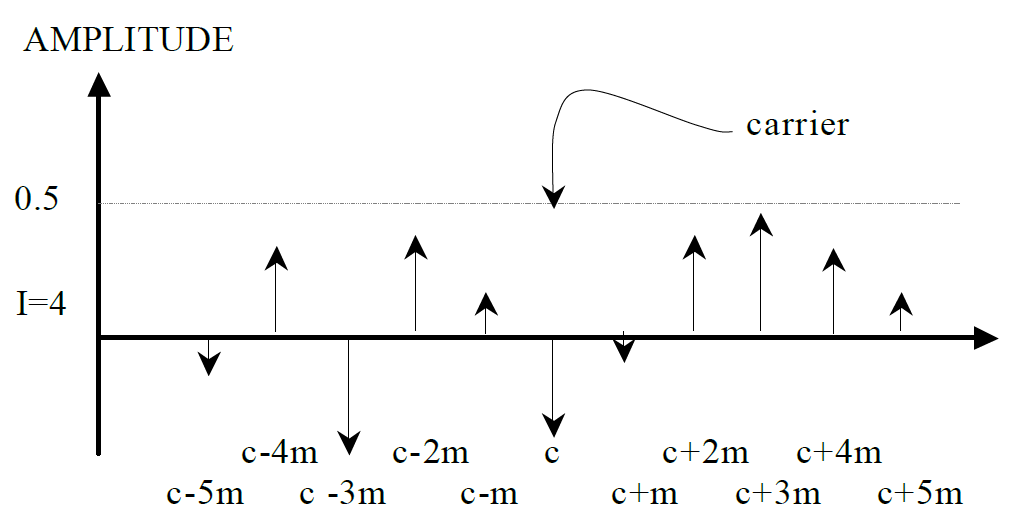
\includegraphics[width=0.4\linewidth]{graficos/EJ4/signos.png}
\caption{Espectro de ejemplo con I=4 e inversiones de fase}
\label{fig:signos}
\end{figure}

\subsection*{Frecuencias laterales reflejadas}
La riqueza de la técnica de modulación en frecuencia yace en que el espectro ubicado en la parte negativa del dominio interfiere con la parte positiva dando lugar a una mezcla de componentes en ambas partes del espectro. La relación entre frecuencias $f_c$ y $f_m$ es la que da origen a un espectro harmónico o uno inharmónico.
\subsection*{Espectro harmónico e inharmónico}
La relación entre frecuencias esta dada por \\*

\begin{eqnarray*}
\displaystyle \frac{f_c}{f_m}=\frac{N_1}{N_2} 
\end{eqnarray*}
 
\begin{eqnarray*}
\displaystyle f_0=gcd(f_c,f_m)
\end{eqnarray*}
 
La posición de las frecuencias laterales en serie harmónica puede ser determinada por las siguientes relaciones

\begin{eqnarray*}
\displaystyle k = N_1 \pm nN_2 \: para\; n=0,1,2,3,4...
\end{eqnarray*}
Donde k es el  número de harmónico y n es el orden de la frecuencia lateral.
Excepto para n=0, k toma dos valores por cada orden.

A continuación dejamos unas generalizaciones útiles:
\begin{itemize}
\item La portadora es siempre el $N_1$-ésimo harmónico  en la serie
\item Si $N_2$ = 1 el espectro contiene todos los harmonicos	y el fundamental es la frecuencia de la modulante
\item Si $N_2$ es un numero par el espectro tiene solo harmónicos impares
\item Si $N_2$ = 3 cada tercer harmónico no se encuentra más en la serie
\end{itemize}
 

El número de harmónicos que tienen amplitud significativa  dependen del índice de modulación.

Para relaciones entre frecuencias bajas e indices chicos donde $N_1\neq1$ la fundamental puede no estar presente en el espectro.

\begin{figure}[H]
\centering
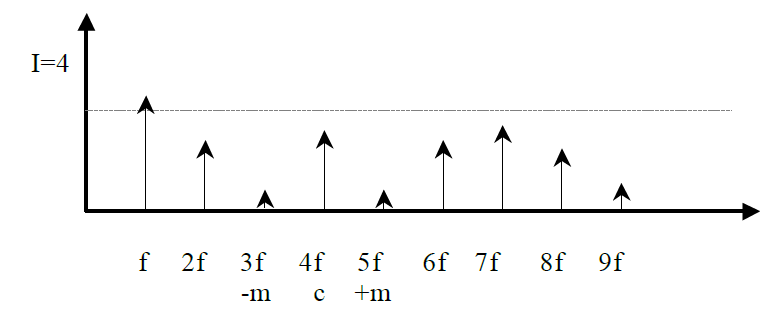
\includegraphics[width=0.5\linewidth]{graficos/EJ4/espectroharmonico.png}
\caption{Espectro donde la relacion $\displaystyle \frac{f_c}{f_m}=\frac{4}{1}$ (harmónico) con I=4 }
\label{fig:harmonico}
\end{figure}

\begin{figure}[H]
\centering
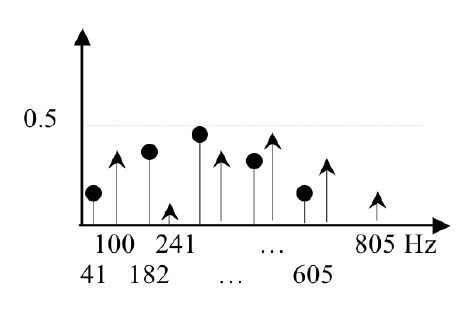
\includegraphics[width=0.3\linewidth]{graficos/EJ4/espectroinharmonico.png}
\caption{Espectro donde la relacion $\displaystyle \frac{f_c}{f_m}=\frac{1}{\sqrt{2}}$ (inharmónico) con I=4}
\label{fig:inharmonico}
\end{figure}

\begin{figure}[H]
\centering
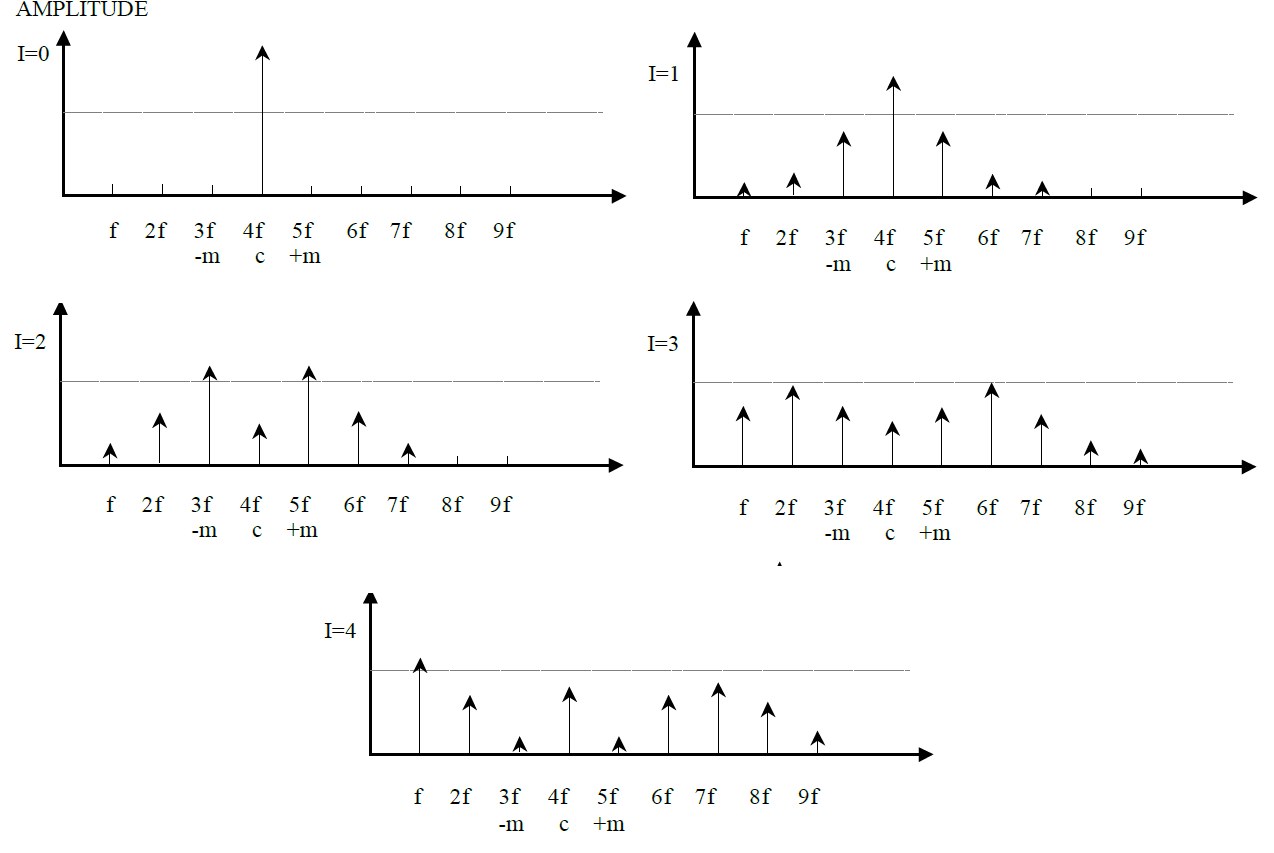
\includegraphics[width=0.8\linewidth]{graficos/EJ4/chowning.png}
\caption{Espectros con distintos índices de modulación (cociente racional)}
\label{fig:chowning}
\end{figure}


%La fundamental solo se vuelve significante cuando I$>$2.\\*
Resumen:\\*
El espectro inharmónico se origina cuando el cociente $\displaystyle \frac{f_c}{f_m}$ da como resultado un número irracional. \\*
El índice de modulación $\displaystyle \frac{f_d}{f_m}$ determina el número de componentes que van a tener amplitud significante.

\subsection{Espectro dinámico}
La complejidad del espectro esta relacionada con el índice de modulación de forma tal que si el indice crece el bandwidth también crece. Entonces si pensamos en un índice de modulación que varía con el tiempo la evolución del bandwidth del espectro puede estar generalmente descrita por la forma de la función.
No obstante, la evolución de cada componente es determinado por la forma de la funcion de Bessel correspondiente.
Entonces, si el indice de modulación aumenta con el tiempo el bandwidth también lo hace, pero un componente del espectro va a crecer o decrecer en amplitud dependiendo de la pendiente de la función de bessel en ese rango de indices.

\begin{figure}[H]
\centering
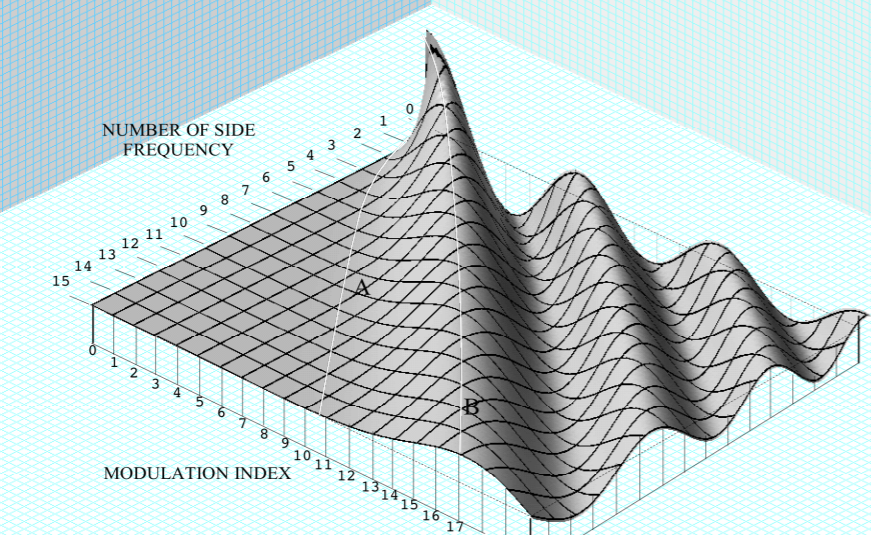
\includegraphics[width=0.8\linewidth]{graficos/EJ4/EspectroDinamico.png}
\caption{Funciones de Bessel desde $J_0$ hasta $J_{15}$ e I desde 0 hasta 20. En este gráfico se puede ver rápidamente el bandwidth dado un índice I}
\label{fig:DynamicSpectrum}
\end{figure}



\subsection{Síntesis para instrumentos de viento}
Para los intrumentos de viento:
\begin{eqnarray*}
\displaystyle \phi_m=\phi_c=-\frac{\pi}{2}
\end{eqnarray*}
Resultando
\begin{eqnarray*}
\textstyle x(t)=\textcolor{red}{A(t)}\cdot sen(2\pi f_c t+\textcolor{orange}{I(t)}\cdot sen(2\pi f_mt))
\end{eqnarray*}

\subsubsection{Síntesis de clarinete}
%Para un clarinete se utiliza un esquema similar al ADSR con %Attack Sustain y Release. En lugar de tratarse de una %interpolación lineal entre puntos, se trata de una %interpolación exponencial.
Para poder sintetizar un clarinete se establecieron los parámetros recomendados por la literatura
 
\begin{eqnarray*}
\displaystyle \frac{f_c}{f_m}=\frac{2}{3}
\end{eqnarray*}

Las envolventes sugeridas por la bibliografía poseen la siguiente forma
\begin{figure}[H]
\centering
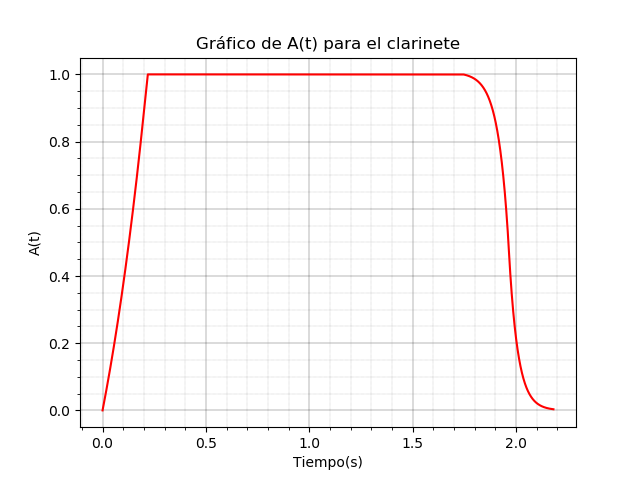
\includegraphics[width=0.4\linewidth]{graficos/EJ4/at_clarinet.png}
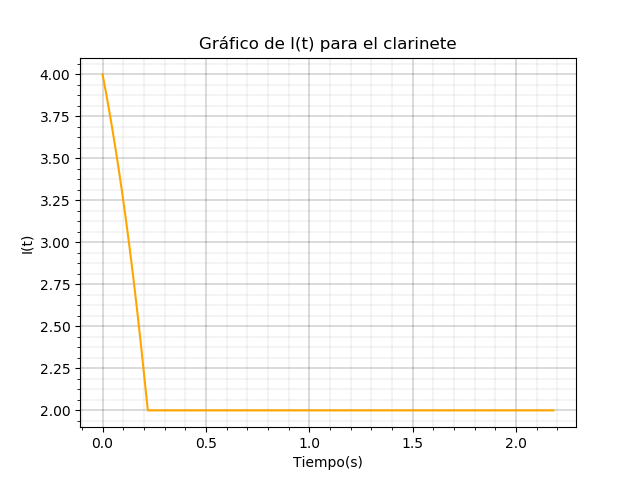
\includegraphics[width=0.4\linewidth]{graficos/EJ4/it_clarinet.png}
\caption{A(t) e I(t) respectivamente}
\label{fig:clarinet_envelopes}
\end{figure}

\begin{figure}[H]
\centering
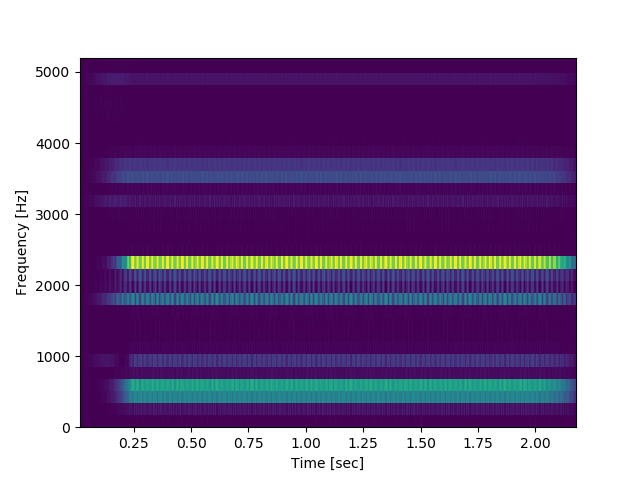
\includegraphics[width=0.4\linewidth]{graficos/EJ4/ClarinetEspectogram440Hz.png}
\caption{Espectrograma de la síntesis del clarinete a 440Hz (nota LA)}
\label{fig:clarinet_440}
\end{figure}


\subsubsection{Síntesis de campana}
Parámetros recomendados por la literatura para la síntesis:
\begin{eqnarray*}
\displaystyle \frac{f_c}{f_m}=\frac{2}{1}
\end{eqnarray*}
Envolventes sugeridos:
\begin{figure}[H]
\centering
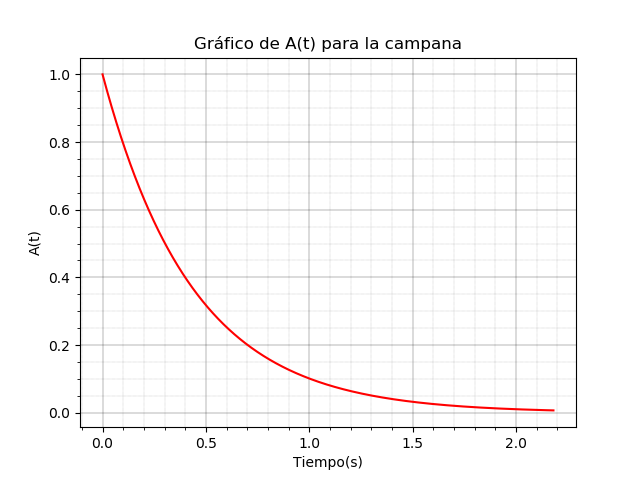
\includegraphics[width=0.4\linewidth]{graficos/EJ4/at_bell.png}
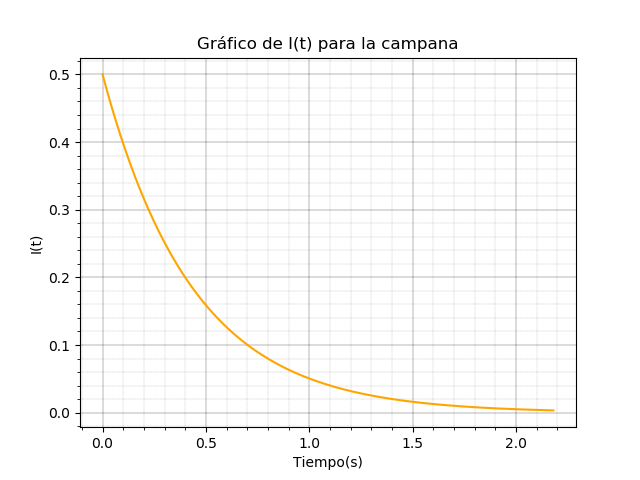
\includegraphics[width=0.4\linewidth]{graficos/EJ4/it_bell.png}
\caption{A(t) e I(t) respectivamente}
\label{fig:bell_envelopes}
\end{figure}

\begin{figure}[H]
\centering
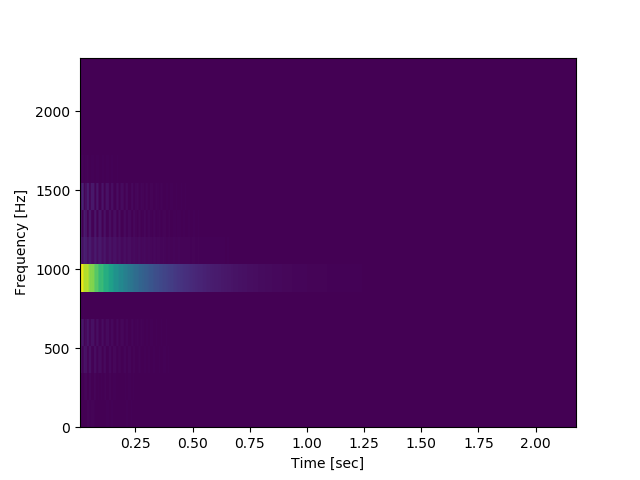
\includegraphics[width=0.4\linewidth]{graficos/EJ4/BellEspectogram440Hz.png}
\caption{Espectrograma de la síntesis de la campana a 440Hz (nota LA)}
\label{fig:bell_440}
\end{figure}
\subsubsection{Síntesis de trombón}
Para los Brass Instruments se recomienda utilizar una relación de:
\begin{eqnarray*}
\displaystyle \frac{f_c}{f_m}=\frac{1}{1}
\end{eqnarray*}

\begin{figure}[H]
\centering
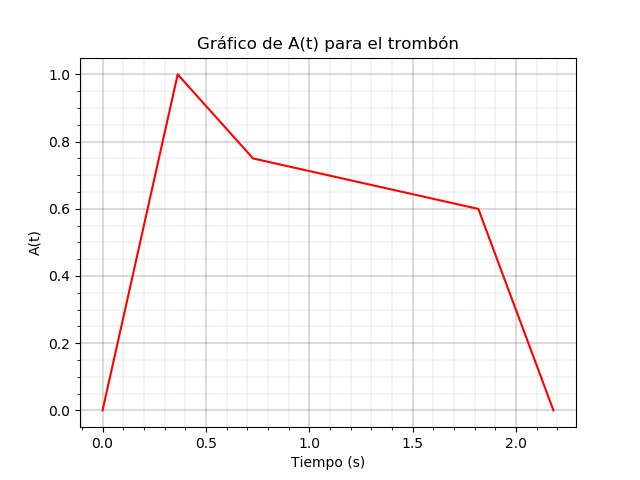
\includegraphics[width=0.4\linewidth]{graficos/EJ4/at_trombon.png}
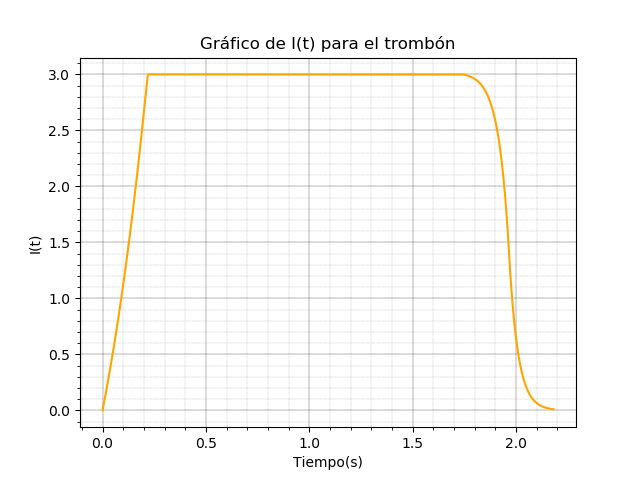
\includegraphics[width=0.4\linewidth]{graficos/EJ4/it_trombon.png}
\caption{A(t) e I(t) respectivamente}
\label{fig:trombone_envelopes}
\end{figure}

\begin{figure}[H]
\centering
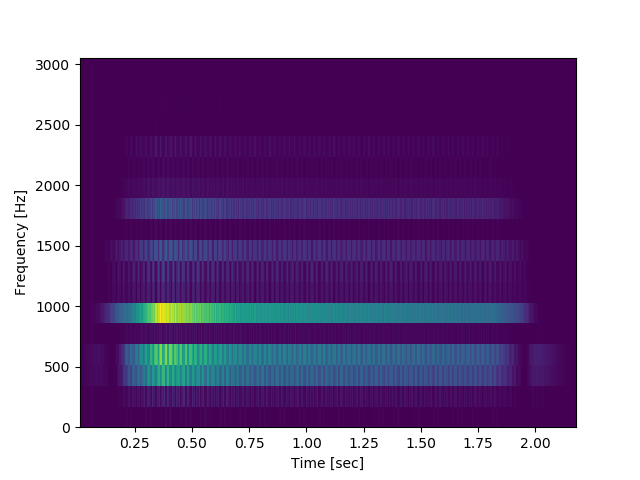
\includegraphics[width=0.4\linewidth]{graficos/EJ4/espectrograma_trombon.png}
\caption{Espectrograma de la síntesis del trombón a 440Hz (nota LA)}
\label{fig:trombone_440}
\end{figure}

\subsection{Conclusiones}
Para poder realizar una síntesis de un instrumento suele ser útil tener espectrogramas del mismo ya que nos dan información de cómo evoluciona el sonido con el tiempo y de esa forma se puede llegar a tener una idea de cómo puede llegar a ser A(t) e I(t). Si bien en la literatura hay envolventes sugeridas, las mismas son sólo un molde inicial por el cual uno debería empezar a probar la síntesis pero para poder ejecutar una síntesis apropiada se debe cambiar el molde. De la misma forma la relación entre fm y fc no siempre tiene que ser la sugerida. 
\begin{thebibliography}{9}
  
\bibitem{knuthwebsite} 
The Synthesis of Complex Audio Spectra by Means of Frequency Modulation,
\\\texttt{\url{https://ccrma.stanford.edu/sites/default/files/user/jc/fm_synthesispaper-2.pdf}}

\bibitem{knuthwebsite} 
FM Synthesis for Musical Instruments: Bells and Clarinets,
\\\texttt{\url{http://home.eng.iastate.edu/~julied/classes/ee224/Labs/FMSynthesis_lab.pdf}}
%\url{http://home.eng.iastate.edu/~julied/classes/ee224/Labs/FMSynthesis_lab.pdf}
%\~julied/classes/ee224/Labs/FMSynthesis_lab.pdf

\end{thebibliography}


\end{document}